% Chapter 12 opener diagram: "Visualizing Multivariate Models"
% Center bubble = chapter; satellites = its numbered sections.
% Section list mirrors the chapter .qmd — update here when sections change,
% then rebuild with ./make-diagrams.sh
\documentclass[border=8pt]{standalone}
% diagram-common.tex — shared setup for the part-page and chapter-opener
% bubble diagrams (DDAR style). \input by every part*.tex and chap*.tex in
% this directory. Rebuild all diagrams with ./make-diagrams.sh
%
% Center bubble: strong part accent color (latex/part-colors.tex) with a
% gentle top-lit gradient, white bold sans text, and a thin divider rule
% under the number. Satellites: light tint gradient of the same color,
% black text. All bubbles cast a soft blur shadow. Connections are tapered
% bands shaded dark -> light, drawn as a single path each (the TikZ mindmap
% library's connection bars leave hairline seams between fill segments, so
% we draw our own).
\usepackage[cmyk]{xcolor}   % CRC wants CMYK — same as latex/preamble.tex
\usepackage{amsmath}        % \boldsymbol etc. in section labels
% Part accent colors — change here to retheme the whole book.
% Shared by latex/preamble.tex (section heads, chapter titles, running heads)
% and by latex/diagrams/*.tex (part-page and chapter-opener mindmap diagrams).
% After changing a color, re-run latex/diagrams/make-diagrams.sh so the
% pre-built diagrams in figs/diagrams/ pick up the new colors.
\colorlet{partI}  {blue}
\colorlet{partII} {teal}
\definecolor{partIII}{cmyk}{0.67, 0, 0.43, 0.55}  % #267342
\definecolor{partIV}{cmyk}{0, 0.50, 1.0, 0.20}  % #CC6600 — burnt orange, darker than xcolor's orange

\usepackage{tikz}
\usetikzlibrary{calc, shadows.blur}

% \band{color}{angle}{distance}: tapered connection band from the center
% bubble out to (angle:distance), shaded color -> light tint. Bands are
% drawn before the bubbles, so both ends tuck underneath them.
\newlength\bandroot \setlength\bandroot{0.50cm}  % half-width at the center
\newlength\bandmid  \setlength\bandmid {0.16cm}  % half-width at the waist
\newlength\bandtip  \setlength\bandtip {0.28cm}  % half-width at the satellite
\newcommand\band[3]{%
  \path[shading=axis, bottom color=#1, top color=#1!35, shading angle={#2-90}]
    (#2+90:\bandroot)
      .. controls ($(#2:0.5*#3)+(#2+90:\bandmid)$) .. ($(#2:#3)+(#2+90:\bandtip)$)
    -- ($(#2:#3)+(#2-90:\bandtip)$)
      .. controls ($(#2:0.5*#3)+(#2-90:\bandmid)$) .. (#2-90:\bandroot)
    -- cycle;}

% \bubbletitle{number}{title}: stacked number + divider rule + title for the
% center bubble.
\newcommand\bubbletitle[2]{%
  {\LARGE #1}\\[3.5pt]{\rule{1.05cm}{0.45pt}}\\[5.5pt]#2}

\tikzset{
  softshadow/.style={blur shadow={shadow blur steps=6,
    shadow xshift=0.5mm, shadow yshift=-0.8mm}},
  rootbubble/.style={circle, top color=#1!88!white, bottom color=#1!90!black,
    text=white, align=center, inner sep=1pt,
    font=\sffamily\bfseries, softshadow,
    execute at begin node={\hyphenpenalty=10000 }},
  satbubble/.style={circle, top color=#1!22, bottom color=#1!42,
    text=black, align=center, inner sep=1pt, softshadow,
    execute at begin node={\hyphenpenalty=10000 }},
}

\begin{document}
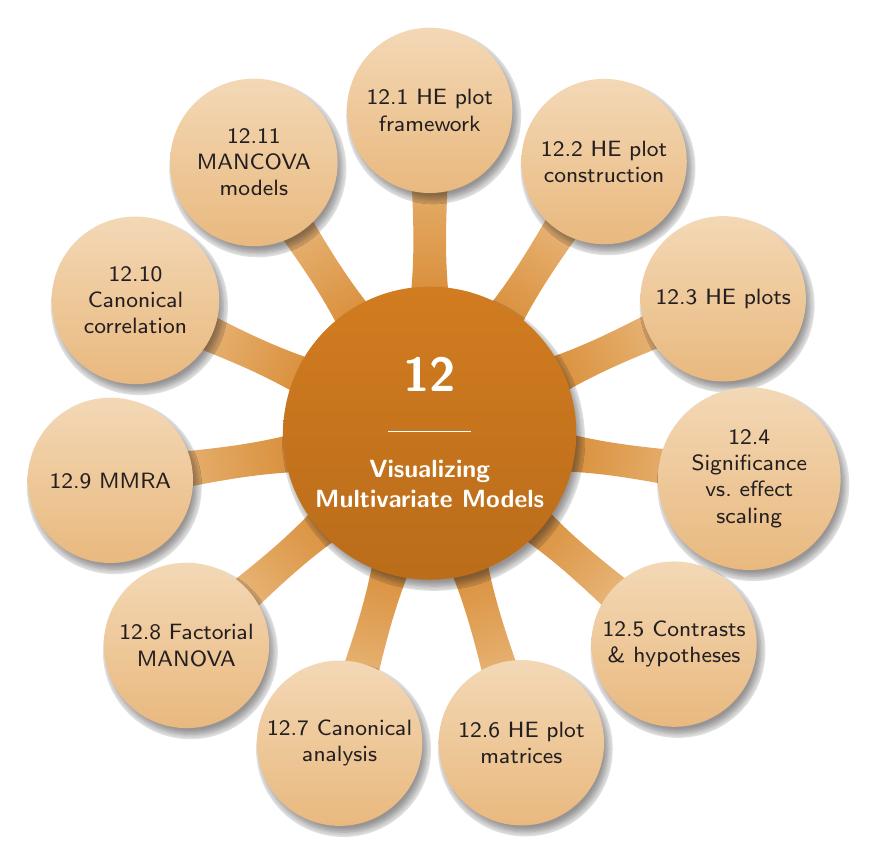
\begin{tikzpicture}[
  sat/.style={satbubble=partIV, minimum size=2.1cm, text width=1.85cm,
              font=\sffamily\footnotesize}]
% connection bands (drawn first; the bubbles cover their ends)
\band{partIV}{90}{4.1}
\band{partIV}{57.3}{4.1}
\band{partIV}{24.6}{4.1}
\band{partIV}{351.9}{4.1}
\band{partIV}{319.2}{4.1}
\band{partIV}{286.5}{4.1}
\band{partIV}{253.8}{4.1}
\band{partIV}{221.1}{4.1}
\band{partIV}{188.4}{4.1}
\band{partIV}{155.7}{4.1}
\band{partIV}{123}{4.1}
% bubbles
\node[rootbubble=partIV, minimum size=3.5cm, text width=3.1cm, font=\sffamily\bfseries\small]
  {\bubbletitle{12}{Visualizing Multivariate Models}};
\node[sat] at (90:4.1) {12.1 HE plot framework};
\node[sat] at (57.3:4.1) {12.2 HE plot construction};
\node[sat] at (24.6:4.1) {12.3 HE plots};
\node[sat] at (351.9:4.1) {12.4 Significance vs.\ effect scaling};
\node[sat] at (319.2:4.1) {12.5 Contrasts \& hypotheses};
\node[sat] at (286.5:4.1) {12.6 HE plot matrices};
\node[sat] at (253.8:4.1) {12.7 Canonical analysis};
\node[sat] at (221.1:4.1) {12.8 Factorial MANOVA};
\node[sat] at (188.4:4.1) {12.9 MMRA};
\node[sat] at (155.7:4.1) {12.10 Canonical correlation};
\node[sat] at (123:4.1) {12.11 MANCOVA models};
\end{tikzpicture}
\end{document}
